% When using TeXShop on the Mac, let it know the root document. The following must be one of the first 20 lines.
% !TEX root = ../design.tex

\chapter{Abstraction Layers}

\begin{moduleinfo}
\item[Author] Florian Schoppmann
\item[History]
	\begin{modulehistory}
		\item[v0.6] Replaced UML figure [Rahul Iyer]
		\item[v0.5] Initial revision of design document
		\item[v0.4] Support for function pointers and sparse-vectors
		\item[v0.3] C++ abstraction layer rewritten as a template library, switched to Eigen \cite{eigen} as linear-algebra library
		\item[v0.2] Initial revision of C++ abstraction layer, incorporated Armadillo \cite{armadillo} as linear-algebra library
	\end{modulehistory}
\end{moduleinfo}

% Abstract. What is the problem we want to solve?

\section{The C++ Abstraction Layer}

There are a number of complexities involved in writing C or C++-based user-defined functions over a legacy DBMS like PostgreSQL, all of which can get in the way of maintainable, portable application logic. This complexity can be especially frustrating for routines whose pseudocode amounts to a short linear-algebra expression that \emph{should} result in a compact implementation.

MADlib provides a C++ abstraction layer both to ease the burden of writing high-performance UDFs, and to encapsulate DBMS-specific logic inside the abstraction layer, rather than spreading the cost of maintenance and porting across all the UDFs in the library. In brief, the MADlib C++ abstraction currently provides five classes of functionality: type bridging, math-library integration, resource-management shims, high-level types, and templates for modular fold/reduce components.

\subsection{Overview of Functionality} \label{sec:C++AL:Classes}

\paragraph{Type Bridging}

The basic responsibility for the C++ abstraction layer is to bridge database types to native C++ types. For a DBMS, a user-defined function implemented in a compiled language is typically nothing more but a symbol (i.e., an address) in a shared library. As such, DBMS APIs specify that UDFs must have a fixed signature, and arguments are passed as an array of pointers along with additional meta data. Hand-written C code would therefore often consist of long boilerplate code that is very specific to the underlying DBMS: Making sure that the passed data is of the correct type, copying immutable data before doing modifications, verifying array lengths, etc. The C++ abstraction layer encapsulates all this within the recursive \texttt{AnyType} class that can contain either a primitive type (like, e.g., \texttt{int} or \texttt{double}) or multiple other values of type \texttt{AnyType} (for representing a composite type). This encapsulation works both for passing data from the DBMS to the C++ function, as well as returning values back from C++. To give an example: A simple, portable, and completely type-safe (though arguably not very useful) function that adds two numbers could be implemented with essentially as little code as in a high-level scripting language:
\begin{cpp}
    AnyType
    sum_two_doubles::run(AnyType& args) {
        return args[0].getAs<double>()
             + args[1].getAs<double>();
    }
\end{cpp}

\paragraph{Math-Library Integration and Performance}

SQL comes without any native support for vector and matrix operations. This presents challenges at two scales. At a macroscopic level, matrices must be intelligently partitioned into chunks that can fit in memory on a single node. At a microscopic scale, the database engine must invoke efficient linear-algebra routines on the pieces of data it gets in core. To this end, the C++ abstraction layer incorporates the very performant linear-algebra library Eigen~\cite{eigen}. Most importantly, it provides additional type bridges that do not involve memory copying and thus are very efficient: For instance, double-precision arrays in the DBMS are the canonic way to represent real-valued vectors. Therefore, the C++ abstraction layer not just provides an array-to-array bridge but also maps DBMS arrays to Eigen vectors. The bridged types can be used with all of the very sophisticated vector and matrix operations provided by Eigen.

Incorporating proven third-party libraries moreover makes it easy for MADlib developers to write correct and performant code: For instance, the Eigen linear-algebra library contains well-tested and well-tuned code that makes use of the SIMD instruction sets (like SSE) found in today's CPUs. Recent versions of Eigen even allow coupling with proprietary high-performance mathematical routines like the Intel Math Kernel Library.

Likewise, the C++ abstraction layer itself has been tuned for efficient value marshaling. Some examples include: All type bridges are aware of mutable and immutable objects and avoid making copies whenever possible. DBMS-catalogue lookups occur only once per query and are then minimized by caching. Moreover, the C++ abstraction layer is written as a template library and with the goal of reducing the runtime and abstraction overhead to a minimum. In particular, it takes extra steps to avoid memory allocation whenever possible.

\paragraph{Resource-Management Shims}

Another aspect of the C++ abstraction layer is to provide a safe and robust runtime environment with a standard interface. For instance, PostgreSQL maintains a hierarchy of memory contexts: When a query is started, a new memory context is created and all transient memory allocations are supposed to occur within this context. When the query ends, disposing of the query context provides a simple and effective way of garbage collection. The C++ abstraction layer makes sure that such modi operandi are followed. On the other hand, the C++ abstraction layer also facilitates writing C++ code with a well-defined interface. This is particularly necessary if (as is typically the case) a DBMS only provides a C plugin interface: In that case it is important that exceptions, signals, etc.\ do not cross runtime boundaries.

\paragraph{High-level types}

A second responsibility of the abstraction layer is to help compensating for SQL's lack of higher-order logic: For instance, an \texttt{AnyType} object can contain a \texttt{FunctionHandle}, which points to a user-defined function. With the syntactic sugar possible in C++, this essentially makes in-database functions first-class objects like they commonly are in modern programming languages. Internally, the abstraction layer maps UDFs to their object ID in the database, and it takes care of looking up the function in the database catalog, verifying argument lists, ensuring type-safety, etc.

Likewise, there is the need to pass internal data structures from one UDF to another (i.e., possibly through the DBMS) in a performant and portable way. While DBMSs like PostgreSQL support user-defined composite types, converting into them (or even using them in internal C++ code) is slow, creates dependencies on MADlib-specific type-bridging classes, and hinders code reuse in/from other projects than MADlib. The C++ abstraction layer therefore contains the recursive \ref{sym:DynamicStruct} class that provides a C++ struct/class interface around a stream of bytes. This class is very generic and can easily be used with any contiguous blocks of memory. Compared to the alternative of using existing serialization and deserialization classes, we expect \ref{sym:DynamicStruct} to be far better performing, as it modifies constant-length elements directly in the byte stream.

\paragraph{Modular Fold/Reduce Components}

The most basic building block in the macro-programming of MADlib is the use of user-defined aggregates (UDAs). In general, aggregates---and the related window functions---are the natural way in SQL to implement mathematical functions that take as input the values of an arbitrary number of rows. Unfortunately, concrete extension interfaces for user-defined aggregates vary widely across vendors and open-source systems. Nonetheless, the aggregation paradigm (or in functional programming terms, ``fold and reduce'') is natural and ubiquitous, and in most widely-used DBMSs (e.g., in PostgreSQL, MySQL, Greenplum, Oracle, SQL Server, Teradata) a user-defined aggregate consists of a well-known pattern of two or three user-defined functions:
\begin{enumerate}
	\item A \emph{transition function} that takes the current transition state and a new data point. It combines both into into a new transition state. The transition function is equivalent to the ``combining'' function passed to linear \emph{left-fold} functions in functional-programming languages.
	\item An optional \emph{merge function} that takes two transition states and computes a new combined transition state. This function is only needed for parallel execution. In functional-programming terms, a merge operation is a tree-like fold.
	\item A \emph{final function} that takes a transition state and transforms it into the output value.
\end{enumerate}
Clearly, a user-defined aggregate is inherently data-parallel if the transition function is associative and the merge function returns the same result as if the transition function was called repeatedly for every individual element in the second state.

Since the fold/reduce computational model is so ubiquitous and we anticipate the need to share code with other projects, fold/reduce code should not be interwoven with the DBMS interface. That is, fold/reduce-components should be implemented as independent C++ classes (possibly as generic template classes), without dependencies on MADlib-specific type-bridging classes like \texttt{AnyType}. However, fold/reduce components need to store their state as objects that the backend can understand---for maximum portability, all state information must even reside in a single contiguous block of memory. The C++ abstraction layer therefore provides a recursive class \texttt{DynamicStruct} that can contain objects both of primitive data types as well as objects of variable length, including other objects of \texttt{DynamicStruct}. This solution is more performant than serialization and deserialization, because it allows fixed-length datums to be modified directly in the block of memory.


\subsection{Type Bridging}

\subsubsection[Class AnyType]{Class \symlabel{AnyType}{sym:AnyType}}

\ref{sym:AnyType} is a container type for all values that are passed between the DBMS and C++ code. This also includes values passed to or returned from UDFs invoked as \ref{sym:FunctionHandle}. An \ref{sym:AnyType} object represents one of three kinds of values:
%
\begin{enumerate}
	\item NULL
	\item A simple value. E.g., this may be a value of a primitive data type like \texttt{int} or \texttt{double}, or a value of some abstraction-layer type like \ref{sym:FunctionHandle}.
	\item A composite value (i.e., a tuple). In this case, the \ref{sym:AnyType} object contains a list of other \ref{sym:AnyType} objects. Tuple elements are not named but instead accessed by index.
\end{enumerate}
%
\ref{sym:AnyType} objects should be explicitly instantiated only for returning values to the backend or for invoking a \ref{sym:FunctionHandle}. Implementations may choose to have different internal representations for values received from the backend and values from UDF code. The two constructors below only pertain to instantiations within UDF code. Constructors used by internal abstraction-layer code are implementation-specific.

\paragraph{Member functions}

\begin{itemize}
	\item
		\begin{cppsnippet}
		AnyType()
		\end{cppsnippet}

		Default constructor. Initializes this object as NULL. This constructor must also be used for initializing a composite object. After construction, \texttt{operator<\/<()} can be used to append values to the composite object.

	\item
		\begin{cppsnippet}
		template <class T> AnyType(const T& inValue)
		\end{cppsnippet}

		Template constructor (will not be used as copy constructor). This constructor will be invoked when initializing this object with an arbitrary value (excluding composite types).

	\item
		\begin{cppsnippet}
		template <class T> T getAs()
		\end{cppsnippet}

		Convert this object to the type specified as template argument.

	\item
		\begin{cppsnippet}
		AnyType operator[](uint16_t inID) const
		\end{cppsnippet}

		If this object is a composite value, return the element with index \texttt{inID}. To the user, \ref{sym:AnyType} is a fully recursive type: An \ref{sym:AnyType} object may contain a composite value, in which case it is composed of a number of other AnyType objects.

		This method will raise an error if this object does not contain a composite value.

	\item
		\begin{cppsnippet}
		uint16_t numFields() const
		\end{cppsnippet}

		Return the number of elements in the tuple. If this object contains NULL, return 0; if it contains a simple value, return 1.

	\item
		\begin{cppsnippet}
		bool isNull() const
		\end{cppsnippet}

		Return if this object is NULL.

	\item
		\begin{cppsnippet}
		bool isComposite() const
		\end{cppsnippet}

		Return if this object is a composite value.

	\item
		\begin{cppsnippet}
		AnyType& operator<<(const AnyType& inValue)
		\end{cppsnippet}

		If this object is NULL, or a composite value that has previously been constructed with the default constructor, add an element to this object. Otherwise, raise an error.
\end{itemize}

\paragraph{Non-Member Functions}

\begin{itemize}
	\item
		\begin{cppsnippet}
		AnyType Null()
		\end{cppsnippet}

		Return an AnyType object representing NULL.

	\item
		\begin{cppsnippet}
		template <class T> T AnyType_cast(const AnyType& inValue)
		template <class T> T AnyType_cast(const T& inValue)
		template <class T> T AnyType_cast(T& inValue)
		\end{cppsnippet}

		Explicit cast that converts \ref{sym:AnyType} objects to a target type \texttt{T}, but leaves values that already are of type \texttt{T} unaffected.

		Sometimes it is desirable to write generic code that works on both an \ref{sym:AnyType} object as well as a value with a concrete type. For instance, a \ref{sym:FunctionHandle} always returns an \ref{sym:AnyType} object. In generic code, however, a \ref{sym:FunctionHandle} might as well be replaced by just a call to a ``normal'' functor or a C++ function pointer, both of which typically return concrete types (e.g., \texttt{double}).

		In generic code, we could write \texttt{AnyType\_cast<double>(func())} so that if the template type of \texttt{func} is a \ref{sym:FunctionHandle}, we have an explicit conversion to \texttt{double}, whereas if \texttt{func} is just a function pointer, the return value of \texttt{func()} passes unchanged.
\end{itemize}


\subsection{Math-Library Integration}

\subsubsection[Class HandleMap]{Class \symlabel{HandleMap}{sym:HandleMap}}

\paragraph{Requirements}

\begin{itemize}
	\item \texttt{EigenType} The Eigen type that this \ref{sym:HandleMap} will wrap. Examples are \texttt{Eigen::VectorXd} or \texttt{Eigen::MatrixXd}.
	\item \texttt{Handle} Type conforming to \ref{sym:ContiguousDataHandle} concept. The two types \texttt{EigenType::Scalar} and \texttt{Handle::element\_type} must coincide.
	\item \texttt{MapOptions} Passed as template parameter \texttt{MapOptions} to \texttt{Eigen::Map}.
\end{itemize}

\paragraph{Types}

\begin{itemize}
	\item \texttt{Index}: \texttt{EigenType::Index}
\end{itemize}

\paragraph{Member functions}

\begin{itemize}
	\item
		\begin{cppsnippet}
		// constructors
		HandleMap(const Handle& inHandle) // (1)
		HandleMap(const Eigen::MapBase<Derived>& inMappedData) // (2)
		HandleMap(const Handle &inHandle, Index inNumElem) // (3)
		HandleMap(const Handle &inHandle, Index inNumRows, Index inNumCols) // (4)
		\end{cppsnippet}

		Constructor (1) constructs an empty \ref{sym:HandleMap} that points to NULL. Constructor (2) constructs a \ref{sym:HandleMap} that is backed by a contiguous memory block within an existing Eigen matrix (or vector). Note that not all of Eigen's block operations return contiguous memory blocks. E.g., while the \texttt{col()} method returns contiguous blocks if column-oriented storage is used, the \texttt{row()} method does not! Constructor (3) and (4) construct a \ref{sym:HandleMap} that is backed by a \texttt{Handle}.

	\item
		\begin{cppsnippet}
		HandleMap& operator=(const HandleMap& other)
		\end{cppsnippet}

		Assign another \ref{sym:HandleMap} to this object. This does not change any references or pointers, but copies all elements, i.e., the behavior is identical to other Eigen objects.

	\item
		\begin{cppsnippet}
		HandleMap& rebind(const Handle& inHandle);
		HandleMap& rebind(const Handle& inHandle, Index inSize);
		HandleMap& rebind(const Handle& inHandle, Index inRows, Index inCols);
		HandleMap& rebind(Index inSize);
		HandleMap& rebind(Index inRows, Index inCols);
		\end{cppsnippet}

		Change the handle that is backing this object. All except the first form may also be used to change the dimensions of the matrix (or vector) represented by this object.
\end{itemize}

\paragraph{Concrete Types}

\begin{itemize}
	\item \texttt{MappedMatrix}: \texttt{HandleMap<const Matrix, TransparentHandle<double> >}
	\item \texttt{MutableMappedMatrix}: \texttt{HandleMap<Matrix, TransparentHandle<double, Mutable> >}
	\item \texttt{NativeMatrix}: \texttt{HandleMap<const Matrix, ArrayHandle<double> >}
	\item \texttt{MutableNativeMatrix}: \texttt{HandleMap<Matrix, MutableArrayHandle<double> >}
	\item The corresponding four definitions for \texttt{ColumnVector} instead of \texttt{Matrix}.
\end{itemize}


\subsection{Resource-Management Shims}

\subsubsection[Class Allocator]{Class \symlabel{Allocator}{sym:Allocator}}

\paragraph{Member functions}

\subsubsection[Class NativeRandomNumberGenerator]{Class \symlabel{NativeRandomNumberGenerator}{sym:NativeRandomNumberGenerator}}

\paragraph{Member functions}


\subsection{High-Level Types}

\subsubsection[Class FunctionHandle]{Class \symlabel{FunctionHandle}{sym:FunctionHandle}}

A \ref{sym:FunctionHandle} is a function ``pointer'' to a UDF. A compliant implementation might just store the object ID of the UDF in the database, and upon invocation look up the function in the database catalog, do argument verification, retrieve a function pointer in memory and finally invoke this function pointer.

There are several options for implementations to improve performance. First, if function \texttt{funcPtr()} returns a non-NULL value, the UDF is implemented using the C++ abstraction layer and can be called directly, without going through the usual backend functions. Second, the \texttt{invoke} function is \emph{not} \texttt{const}, so implementations can cache metadata (and therby modify the \ref{sym:FunctionHandle} object).

\paragraph{Types}

\begin{itemize}
	\item
		\texttt{udf\_ptr}: \texttt{AnyType (*)(AnyType\&)}
\end{itemize}

\paragraph{Member functions}

\begin{itemize}
	\item
		\begin{cppsnippet}
		udf_ptr funcPtr();
		\end{cppsnippet}

		If the UDF is a function written using the C++ abstraction layer, implementations may return a pointer to the C++ function. Alternatively, an implementation may always return NULL. Callers must not rely on \texttt{funcPtr} returning non-NULL values.

	\item
		\begin{cppsnippet}
		FunctionHandle& setFunctionCallOptions(uint32_t inFlags)
		FunctionHandle& unsetFunctionCallOptions(uint32_t inFlags)
		uint32_t getFunctionCallOptions() const
		\end{cppsnippet}

		Set or get the current function call options. Options are a bit field of properties as defined above.

	\item
		\begin{cppsnippet}
		AnyType invoke(AnyType& args)
		\end{cppsnippet}

		Invoke the UDF with the given arguments. Note that \texttt{args} has to be a composite value.

	\item
		\begin{cppsnippet}
		AnyType operator()()
		AnyType operator()(AnyType& arg1, ..., AnyType& argn)
		\end{cppsnippet}

		Convenience method. Call \texttt{invoke} with the given arguments combined into one composite value.
\end{itemize}


\subsubsection[Concept ContiguousDataHandle]{Concept \symlabel{ContiguousDataHandle}{sym:ContiguousDataHandle}}

A \ref{sym:ContiguousDataHandle} is an opaque pointer to contiguous data that may be augmented by metadata. For instance, a \ref{sym:ContiguousDataHandle} may wrap a DBMS-native array that contains both a pointer to the array data, as well as information about the array's size. Since elements are stored contiguously, they can also be accessed using offsets on regular pointers to elements.

\paragraph{Requirements}

\begin{itemize}
	\item \texttt{T} Element type
\end{itemize}

\paragraph{Types}

\begin{itemize}
	\item
		\texttt{element\_type}: \texttt{T}
\end{itemize}

\paragraph{Member Functions}

\begin{itemize}
	\item
		\begin{cppsnippet}
		const element_type* ptr() const
		\end{cppsnippet}

		Return a pointer to the first element.

	\item
		\begin{cppsnippet}
		const element_type& operator[](size_t inIndex) const
		\end{cppsnippet}

		Return an element.
\end{itemize}

\paragraph{Specialized Concepts}

The concept \symlabel{MutableContiguousDataHandle}{sym:MutableContiguousDataHandle} contains also the following non-const member functions:
%
\begin{itemize}
	\item
		\begin{cppsnippet}
		element_type* ptr()
		\end{cppsnippet}

	\item
		\begin{cppsnippet}
		element_type& operator[](size_t inIndex)
		\end{cppsnippet}
\end{itemize}
%
The concept \symlabel{SizedContiguousDataHandle}{sym:SizedContiguousDataHandle} contains also the following member function:
%
\begin{itemize}
	\item
		\begin{cppsnippet}
		size_t size() const
		\end{cppsnippet}

		Return the number of elements in this object.
\end{itemize}
%
The concept \symlabel{MutableSizedContiguousDataHandle}{sym:MutableSizedContiguousDataHandle} combines both \ref{sym:MutableContiguousDataHandle} and \ref{sym:SizedContiguousDataHandle}.

\subsubsection[Class Ref]{Class \symlabel{Ref}{sym:Ref}}

\ref{sym:Ref} objects are conceptually equivalent to normal C++ references. However, they allow \emph{rebinding} to a different target.

\paragraph{Requirements}

\begin{itemize}
	\item \texttt{T} Target type
	\item \texttt{IsMutable} Boolean parameter indicating if objects of this type can be used to modify the target
\end{itemize}

\paragraph{Types}

\begin{itemize}
	\item
		\texttt{value\_type}: \texttt{T}
\end{itemize}

\paragraph{Member Functions}

\begin{itemize}
	\item
		\begin{cppsnippet}
		Ref& rebind(val_type* inPtr)
		\end{cppsnippet}

		Rebind this reference to a different target.

	\item
		\begin{cppsnippet}
		operator const val_type&() const
		\end{cppsnippet}

		Return a const-reference to the target.

	\item
		\begin{cppsnippet}
		const val_type* ptr() const
		\end{cppsnippet}

		Return a const-pointer to the target.

	\item
		\begin{cppsnippet}
		bool isNull() const
		\end{cppsnippet}

		Return if this reference has been bound to a target.
\end{itemize}

If \texttt{IsMutable == true}, then \ref{sym:Ref} also contains the following non-const member functions:

\begin{itemize}
	\item \texttt{operator val\_type\&()}
	\item \texttt{val\_type* ptr()}
\end{itemize}

Moreover it contains:
\begin{itemize}
	\item
		\begin{cppsnippet}
		Ref& operator=(Ref& inRef)
		Ref& operator=(const val_type& inValue)
		\end{cppsnippet}

		Assign the target value of \texttt{inRef} or \texttt{inValue} to the target of this object.

		It is important to define the first assignment operator because C++ will otherwise perform an assignment as a bit-by-bit copy. Note that this default \texttt{operator=} would be used even though there is a conversion path through \texttt{dest.operator=(orig.operator const val\_type\&())}.
\end{itemize}


\subsubsection[Class ByteStream]{Class \symlabel{ByteStream}{sym:ByteStream}}

\ref{sym:ByteStream} objects are similar to \texttt{std::istream} objects in that they are used to \emph{bind} (as opposed to \emph{read} in the case of \texttt{std::istream}) references to positions in byte sequences. \texttt{operator>\/>()} functions are provided for users of \ref{sym:ByteStream} objects. Each \ref{sym:ByteStream} object controls a \ref{sym:ByteStreamHandleBuf}, which in turn controls a block of memory (the storage/buffer) and has a current position.

A \ref{sym:ByteStream} object can be in \emph{dry-run} mode, in which case \texttt{operator>\/>} invocations move the current position, but no rebinding takes place. Dry-run mode is used, e.g., to determine the storage size needed to hold a \ref{sym:DynamicStruct}.

\paragraph{Member Functions}

\begin{itemize}
	\item
		\begin{cppsnippet}
		template <size_t Alignment>
		size_t seek(std::ptrdiff_t inOffset, std::ios_base::seekdir inDir) // (1)
		size_t seek(size_t inPos) // (2)
		size_t seek(std::ptrdiff_t inOffset, std::ios_base::seekdir inDir) // (3)
		\end{cppsnippet}

		Move the current position in the stream. Variant (1) rounds the new position up to the next multiple of \texttt{Alignment}.

	\item
		\begin{cppsnippet}
		size_t available() const
		\end{cppsnippet}

		Return the number of characters between the current position and the end of the stream.

	\item
		\begin{cppsnippet}
		const char_type* ptr() const
		\end{cppsnippet}

		Return a pointer to the beginning of the buffer.

	\item
		\begin{cppsnippet}
		size_t size() const
		\end{cppsnippet}

		Return the size of the buffer.

	\item
		\begin{cppsnippet}
		size_t tell() const
		\end{cppsnippet}

	\item
		\begin{cppsnippet}
		std::ios_base::iostate rdstate() const
		bool eof() const
		\end{cppsnippet}

		Return status information about the stream, in a fashion similar to \texttt{std::istream}.
	\item
		\begin{cppsnippet}
		bool isInDryRun() const
		\end{cppsnippet}

		Return if the stream is in dry-run mode.

	\item
		\begin{cppsnippet}
		template <class T> const T* read(size_t inCount = 1)
		\end{cppsnippet}

		Advance the current position in the buffer to the next address suitable to read a value of type \texttt{T} and return that address.
\end{itemize}

\paragraph{Non-Member Functions}

\begin{itemize}
	\item
		\begin{cppsnippet}
		template <class Reference>
		ByteStream& operator>>(ByteStream& inStream, Reference& inReference)
		\end{cppsnippet}

		Bind a reference to the next suitable address in the buffer. Internally, this function calls \texttt{read<typename Reference::val\_type>(inReference.size())}.
\end{itemize}

\subsubsection[Class ByteStreamHandleBuf]{Class \symlabel{ByteStreamHandleBuf}{sym:ByteStreamHandleBuf}}

\ref{sym:ByteStreamHandleBuf} objects are similar to \texttt{std::streambuf} objects in that they are in charge of providing reading functionality from certain types of byte sequences. Unlike \texttt{std::streambuf}, however, reading refers to \emph{binding} a reference to the current position in the byte sequence.

\ref{sym:ByteStreamHandleBuf} objects are associated with a \emph{storage} objects, which is of a class conforming to the \ref{sym:ContiguousDataHandle} concept.

\paragraph{Types}

\begin{itemize}
	\item \texttt{Storage\_type}: Type conforming to \ref{sym:ContiguousDataHandle} concept.
\end{itemize}

\paragraph{Constants}

\begin{itemize}
	\item \texttt{isMutable}: \texttt{Storage\_type::isMutable}, i.e., \texttt{true} if \texttt{Storage\_type} also conforms to the \ref{sym:MutableContiguousDataHandle} concept, and \texttt{false} if not.
\end{itemize}

\paragraph{Member Functions}

\begin{itemize}
	\item
		\begin{cppsnippet}
		ByteStreamHandleBuf(size_t inSize) // (1)
		ByteStreamHandleBuf(const Storage_type& inStorage) // (2)
		\end{cppsnippet}

		Constructor~(1) constructs an empty buffer initialized with \texttt{inSize} zero characters. Constructor~(2) initializes a buffer using existing storage.

	\item
		\begin{cppsnippet}
		size_t seek(size_t inPos)
		const char_type* ptr() const;
		size_t size() const
		size_t tell() const
		\end{cppsnippet}

		Change the current position in the buffer, return the start of the buffer, return the size of of the buffer, and return the current position in the buffer.
\end{itemize}

The following member functions are only present if \texttt{isMutable == true}.
\begin{itemize}
	\item
		\begin{cppsnippet}
		void resize(size_t inSize, size_t inPivot)
		\end{cppsnippet}

		Change the size of the buffer, and preserve the old buffer in the following way: Denote by $s$ the old size of the buffer, by $n$ the new size \texttt{inSize}, and by $p$ the pivot \texttt{inPivot}. Then bytes $[0, p)$ will remain unchanged, bytes $[p, p + n - s)$ will be initialized with 0, and bytes $[p + (n - s), s + (n - s))$ will contain the old byte range $[p, s)$.
\end{itemize}


\subsubsection[Concept DynamicStructContainer]{Concept \symlabel{DynamicStructContainer}{sym:DynamicStructContainer}}

A \ref{sym:DynamicStructContainer} may contain member variables of type \ref{sym:DynamicStruct}. In order for automatic inclusion in the byte stream of a \ref{sym:DynamicStruct}, the \ref{sym:DynamicStructContainer} has to be provided has the \texttt{Container} template parameter of the \ref{sym:DynamicStruct}.

\paragraph{Types}

\begin{itemize}
	\item \texttt{RootContainer\_type}: Type conforming to \ref{sym:DynamicStructContainer} concept
	\item \texttt{Storage\_type}: Type conforming to \ref{sym:ContiguousDataHandle} concept.
	\item \texttt{ByteStream\_type}: A \ref{sym:ByteStream} class
\end{itemize}

\paragraph{Constants}

\begin{itemize}
	\item \texttt{isMutable}: \texttt{Storage\_type::isMutable}, i.e., \texttt{true} if \texttt{Storage\_type} also conforms to the \ref{sym:MutableContiguousDataHandle} concept, and \texttt{false} if not.
\end{itemize}

\paragraph{Member functions}

\begin{itemize}
	\item
		\begin{cppsnippet}
		void initialize()
		\end{cppsnippet}

		Initialize the object. The default implementation does nothing.

	\item
		\begin{cppsnippet}
		const RootContainer_type& rootContainer() const
		\end{cppsnippet}

		Return the root-level container.

	\item
		\begin{cppsnippet}
		const Storage_type& storage() const
		\end{cppsnippet}

		Return the storage object.

	\item
		\begin{cppsnippet}
		const ByteStream_type& byteStream() const
		\end{cppsnippet}

		Return the stream object.
\end{itemize}

\paragraph{Specialized Concepts}

The concept \symlabel{MutableDynamicStructContainer}{sym:MutableDynamicStructContainer} also has the non-const member functions:
\begin{itemize}
	\item \texttt{RootContainer\_type\& rootContainer()}
	\item \texttt{RootStorage\_type\& storage()}
	\item \texttt{ByteStream\_type\& byteStream()}
	\item
		\begin{cppsnippet}
		template <class SubStruct>
		void setSize(SubStruct &inSubStruct, size_t inSize)
		\end{cppsnippet}
\end{itemize}
%
Moreover, the types \texttt{RootContainer\_type} and \texttt{Storage\_type} have to conform to the respective \texttt{Mutable} concepts, and \texttt{ByteStream\_type} has to be a mutable \texttt{ByteStream} class.


\subsubsection[Class DynamicStruct]{Class \symlabel{DynamicStruct}{sym:DynamicStruct}}

A \ref{sym:DynamicStruct} gives a C++ struct/class interface to a byte stream. Modifying member variables directly modifies the byte stream, without any need for serialization and deserialization. Member variables may have variable length that may be changed even after object creation. Moreover, \ref{sym:DynamicStruct} is a recursive type in it also allows member variables of type \ref{sym:DynamicStruct}.

\paragraph{Requirements}

\begin{itemize}
	\item \texttt{Derived} Type of the derived class. Used for static polymorphism.
	\item \texttt{Container} Type conforming to \ref{sym:DynamicStructContainer} concept.
\end{itemize}

\paragraph{Types}

\begin{itemize}
	\item \texttt{Init\_type}: \texttt{Storage\_type} if the \texttt{Container\_type} is a root-level container, and \texttt{Container\_type} otherwise.

	This is a convenience definition: While in general a \ref{sym:ContiguousDataHandle} would be initialized with its container, a top-level \ref{sym:DynamicStruct} is initialized directly with a \ref{sym:ContiguousDataHandle} (without having to instantiate a root-level container first).

	\item \texttt{Storage\_type}: Type conforming to \ref{sym:ContiguousDataHandle} concept
	\item \texttt{Container\_type}: Type conforming to \ref{sym:DynamicStructContainer} concept.
	\item \texttt{ByteStream\_type}: \texttt{Container\_type::ByteStream\_type}, i.e., a \ref{sym:ByteStream} class as defined by the container
\end{itemize}

\paragraph{Member Functions}

\begin{itemize}
	\item
		\begin{cppsnippet}
		DynamicStruct(Init_type& inInitialization) // constructor
		\end{cppsnippet}

	\item
		\begin{cppsnippet}
		template <class OtherDerived>
		DynamicStruct& copy(
		    const DynamicStruct<
		        OtherDerived,
		        typename OtherDerived::Container_type
		    >& inOtherStruct)
		\end{cppsnippet}

		Copy the value of \texttt{inOtherStruct} into this object. Copying will be performed bitwise, and all member variables will be rebound afterwards.
\end{itemize}

The following member functions are only present if \texttt{isMutable == true}.
\begin{itemize}
	\item
		\begin{cppsnippet}
		void setSize(size_t inSize)
		\end{cppsnippet}

		Set the size of this object.
\end{itemize}

\paragraph{Non-Member Functions}

\begin{itemize}
	\item
		\begin{cppsnippet}
		ByteStream_type& operator>>(ByteStream_type& inStream, Derived& inStruct)
		\end{cppsnippet}

		Bind \texttt{inStruct} to the byte stream at the current position.
\end{itemize}


\subsection{Modular Fold/Reduce Components}

\subsubsection[Concept Accumulator]{Concept \symlabel{Accumulator}{sym:Accumulator}}

A class implementing the \ref{sym:Accumulator} concept derives from \ref{sym:DynamicStruct} and stores a transition state. It contains methods for adding a new tuple to the transition state (equivalent to the \emph{transition function}) as well as adding a new transition state (equivalent to the \emph{merge function}).

\paragraph{Requirements}

\begin{itemize}
	\item \texttt{Container} Type conforming to \ref{sym:DynamicStructContainer} concept.
\end{itemize}

\paragraph{Types}

Inherited from \ref{sym:DynamicStruct}:
\begin{itemize}
	\item \texttt{Init\_type}: Type passed to constructor. It is only needed to pass through the constructor argument to the \ref{sym:DynamicStruct} base class.
	\item \texttt{ByteStream\_type}: \texttt{Container::ByteStream\_type}, i.e., the concrete \ref{sym:ByteStream} type as defined by \texttt{Container}. A reference of this type is passed to the \texttt{bind()} function.
\end{itemize}

\paragraph{Member Functions}

\begin{itemize}
	\item
		\begin{cppsnippet}
		Accumulator(Init_type& inInitialization) // constructor
		\end{cppsnippet}

		The constructor is expected to call \ref{sym:DynamicStruct}\texttt{::initialize()}, which eventually will call the \texttt{bind()} method.\footnote{Unfortunately, the need for defining an \texttt{initialize()} member cannot be removed. No super class can safely call \texttt{initialize()} because the \ref{sym:Accumulator} object has not been completely constructed at that time, yet.}

	\item
		\begin{cppsnippet}
		void bind(ByteStream_type& inStream)
		\end{cppsnippet}

		Bind all elements of the state to the data in the stream.

		Implementations bind a member variable \texttt{x} to the current position in the stream by running \texttt{inStream >\/> x}. Note that even after running \texttt{operator>\/>()} on a member variable, there is no guarantee yet that the variable can indeed be accessed. Instead, if the end of \texttt{inStream} has been reached, it would still be uninitialized. It is crucial to first check this.

		Provided that this methods correctly lists all member variables, all other methods can, however, rely on the fact that all variables are correctly initialized and accessible.

	\item
		\begin{cppsnippet}
		Accumulator& operator<<(const tuple_type& inTuple)
		\end{cppsnippet}

		Add a new tuple to this transition-state object.

	\item
		\begin{cppsnippet}
		template <class OtherContainer>
		Accumulator& operator<<(const Accumulator<OtherContainer>& inOther)
		\end{cppsnippet}

		Add a new transition state to this transition-state object.

		\texttt{OtherContainer} must conform to the \ref{sym:DynamicStructContainer} concept.

	\item
		\begin{cppsnippet}
		template <class OtherContainer>
		Accumulator& operator=(const Accumulator<OtherContainer>& inOther)
		\end{cppsnippet}

		The assignment operator must be implemented, because the implicit assignment operator is not enough: Whenever the length of the \ref{sym:Accumulator} changes, member variables have to be rebound. The \texttt{copy} method in \ref{sym:DynamicStruct} takes care of this and should be explicitly called instead.

		\texttt{OtherContainer} must conform to the \ref{sym:DynamicStructContainer} concept.
\end{itemize}

\begin{figure}
\begin{center}
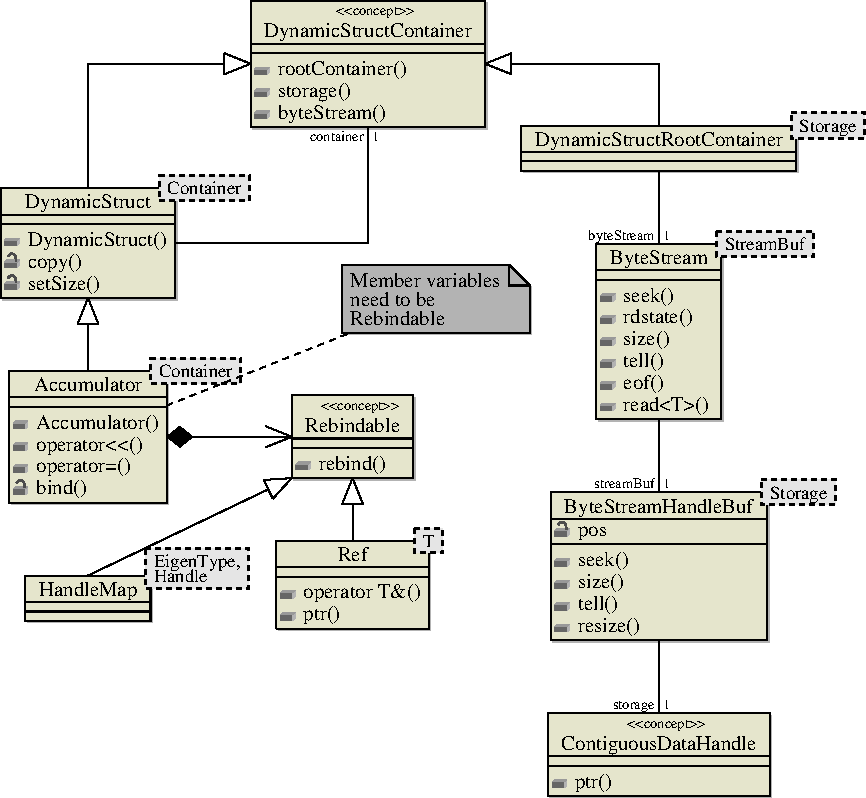
\includegraphics[width=1.1\textwidth]{figures/class_diagram-1}
\end{center}
\caption{Class diagram for modular fold/reduce}
\end{figure}
